%%%%%%%%%%%%%%%%%%%%%%%%%%%%%%%%%%%%%%%%%%%%%%%%%%%%%%%%%%%%%%%%%%%%%%%%%%%%%%%%
%% Plantilla de memoria en LaTeX para la EIF - Universidad Rey Juan Carlos
%%
%% Por Gregorio Robles <grex arroba gsyc.urjc.es>
%%     Grupo de Sistemas y Comunicaciones
%%     Escuela de Ingeniería de Fuenlabrada
%%     Universidad Rey Juan Carlos
%% (muchas ideas tomadas de Internet, colegas del GSyC, antiguos alumnos...
%%  etc. Muchas gracias a todos)
%%
%% La última versión de esta plantilla está siempre disponible en:
%%     https://github.com/gregoriorobles/plantilla-memoria
%%
%% Para obtener PDF, ejecuta en la shell:
%%   make
%% (las imágenes deben ir en PNG o JPG)

%%%%%%%%%%%%%%%%%%%%%%%%%%%%%%%%%%%%%%%%%%%%%%%%%%%%%%%%%%%%%%%%%%%%%%%%%%%%%%%%

\documentclass[a4paper, 12pt]{book}
%\usepackage[T1]{fontenc}

\usepackage[a4paper, left=2.5cm, right=2.5cm, top=3cm, bottom=3cm]{geometry}
\usepackage{times}
\usepackage[utf8]{inputenc}
\usepackage[spanish]{babel} % Comenta esta línea si tu memoria es en inglés
\usepackage{url}
%\usepackage[dvipdfm]{graphicx}
\usepackage{graphicx}
\usepackage{float}  %% H para posicionar figuras
\usepackage[nottoc, notlot, notlof, notindex]{tocbibind} %% Opciones de índice
\usepackage{latexsym}  %% Logo LaTeX

\title{Memoria del Proyecto}
\author{Nombre del autor}

\renewcommand{\baselinestretch}{1.5}  %% Interlineado

\begin{document}

\renewcommand{\refname}{Bibliografía}  %% Renombrando
\renewcommand{\appendixname}{Apéndice}


%%%%%%%%%%%%%%%%%%%%%%%%%%%%%%%%%%%%%%%%%%%%%%%%%%%%%%%%%%%%%%%%%%%%%%%%%%%%%%%%
% PORTADA

\begin{titlepage}
\begin{center}

\includegraphics[scale=0.6]{img/URJ_logo_Color_POS.png}

\vspace{1.75cm}

\LARGE
ESCUELA DE INGENIERÍA DE FUENLABRADA
\vspace{1cm}

\LARGE
TITULACIÓN EN MAYÚSCULAS

\vspace{1cm}
\LARGE
\textbf{TRABAJO FIN DE GRADO/MÁSTER}

\vspace{2cm}

\Large
TÍTULO DEL TRABAJO EN MAYÚSCULAS

\vspace{2cm}

\large
Autor : Nombre del Alumno/a \\
Tutor : Dr. Nombre del Profesor/a\\
Cotutor: (si procede)
\vspace{1cm}

\large
Curso académico 202X/202X

\end{center}
\end{titlepage}

\newpage
\mbox{}
\thispagestyle{empty} % para que no se numere esta pagina



%%%%%%%%%%%%%%%%%%%%%%%%%%%%%%%%%%%%%%%%%%%%%%%%%%%%%%%%%%%%%%%%%%%%%%%%%%%%%%%%
%%%% Para firmar
\clearpage
\pagenumbering{gobble}
\chapter*{}

\vspace{-4cm}
\begin{center}
\LARGE
\textbf{Trabajo Fin de Grado/Máster}

\vspace{1cm}
\large
Título del Trabajo con Letras Capitales para Sustantivos y Adjetivos

\vspace{1cm}
\large
\textbf{Autor :} Nombre del Alumno/a \\
\textbf{Tutor :} Dr. Nombre del Profesor/a

\end{center}

\vspace{1cm}
La defensa del presente Proyecto Fin de Carrera se realizó el día \qquad$\;\,$ de \qquad\qquad\qquad\qquad \newline de 202X, siendo calificada por el siguiente tribunal:


\vspace{0.5cm}
\textbf{Presidente:}

\vspace{1.2cm}
\textbf{Secretario:}

\vspace{1.2cm}
\textbf{Vocal:}


\vspace{1.2cm}
y habiendo obtenido la siguiente calificación:

\vspace{1cm}
\textbf{Calificación:}


\vspace{1cm}
\begin{flushright}
Fuenlabrada, a \qquad$\;\,$ de \qquad\qquad\qquad\qquad de 202X
\end{flushright}

%%%%%%%%%%%%%%%%%%%%%%%%%%%%%%%%%%%%%%%%%%%%%%%%%%%%%%%%%%%%%%%%%%%%%%%%%%%%%%%%
%%%% Dedicatoria

\chapter*{}
\pagenumbering{Roman} % para comenzar la numeracion de paginas en numeros romanos
\begin{flushright}
\textit{Dedicado a \\
mi familia / mi abuelo / mi abuela}
\end{flushright}

%%%%%%%%%%%%%%%%%%%%%%%%%%%%%%%%%%%%%%%%%%%%%%%%%%%%%%%%%%%%%%%%%%%%%%%%%%%%%%%%
%%%% Agradecimientos

\chapter*{Agradecimientos}
%\addcontentsline{toc}{chapter}{Agradecimientos} % si queremos que aparezca en el índice
\markboth{AGRADECIMIENTOS}{AGRADECIMIENTOS} % encabezado 

Este es el fin de una de las etapas más importantes de mi vida y por ello quiero agradecer a varias personas que me han acompañado en este proceso.
Primero quiero agradecer a mi madre Antonia todo el apoyo que me ha dado en cada una de mis decisiones, tanto personales como académicas. Eres quien me impulsa a lograr mis sueños.
Segundo a mi padre Manuel que siempre ha sido mi ejemplo a seguir. Me ha aportado valores fundamentales como el trabajo y el esfuerzo que han sido imprescindibles para abordar esta carrera.
Gracias a los dos por darme la vida.
También agradecer a mi tutor, Gregorio, por darme este proyecto, tener paciencia  y ayudarme en todo cuanto pudo para desarrollarlo.
Por último, quiero agradecer a esa persona tan especial que conocí en esta universidad y que me dio la confianza y la fuerza necesaria para lograr mis metas. 
Paula, gracias por ser mi compañera de viaje y por aparecer en el momento que mas lo necesitaba. Hemos afrontado este desafío juntos y sin ti no hubiera sido igual.


%%%%%%%%%%%%%%%%%%%%%%%%%%%%%%%%%%%%%%%%%%%%%%%%%%%%%%%%%%%%%%%%%%%%%%%%%%%%%%%%
%%%% Resumen

\chapter*{Resumen}
%\addcontentsline{toc}{chapter}{Resumen} % si queremos que aparezca en el índice
\markboth{RESUMEN}{RESUMEN} % encabezado

Aquí viene un resumen del proyecto.
Ha de constar de tres o cuatro párrafos, donde se presente de manera clara y concisa de qué va el proyecto. 
Han de quedar respondidas las siguientes preguntas:

\begin{itemize}
  \item ¿De qué va este proyecto? ¿Cuál es su objetivo principal?
  \item ¿Cómo se ha realizado? ¿Qué tecnologías están involucradas?
  \item ¿En qué contexto se ha realizado el proyecto? ¿Es un proyecto dentro de un marco general?
\end{itemize}

Lo mejor es escribir el resumen al final.

%%%%%%%%%%%%%%%%%%%%%%%%%%%%%%%%%%%%%%%%%%%%%%%%%%%%%%%%%%%%%%%%%%%%%%%%%%%%%%%%
%%%% Resumen en inglés

\chapter*{Summary}
%\addcontentsline{toc}{chapter}{Summary} % si queremos que aparezca en el índice
\markboth{SUMMARY}{SUMMARY} % encabezado

Here comes a translation of the ``Resumen'' into English. 
Please, double check it for correct grammar and spelling.
As it is the translation of the ``Resumen'', which is supposed to be written at the end, this as well should be filled out just before submitting.


%%%%%%%%%%%%%%%%%%%%%%%%%%%%%%%%%%%%%%%%%%%%%%%%%%%%%%%%%%%%%%%%%%%%%%%%%%%%%%%%
%%%%%%%%%%%%%%%%%%%%%%%%%%%%%%%%%%%%%%%%%%%%%%%%%%%%%%%%%%%%%%%%%%%%%%%%%%%%%%%%
% ÍNDICES %
%%%%%%%%%%%%%%%%%%%%%%%%%%%%%%%%%%%%%%%%%%%%%%%%%%%%%%%%%%%%%%%%%%%%%%%%%%%%%%%%

% Las buenas noticias es que los índices se generan automáticamente.
% Lo único que tienes que hacer es elegir cuáles quieren que se generen,
% y comentar/descomentar esa instrucción de LaTeX.

%%%% Índice de contenidos
\tableofcontents 
%%%% Índice de figuras
\cleardoublepage
%\addcontentsline{toc}{chapter}{Lista de figuras} % para que aparezca en el indice de contenidos
\listoffigures % indice de figuras
%%%% Índice de tablas
%\cleardoublepage
%\addcontentsline{toc}{chapter}{Lista de tablas} % para que aparezca en el indice de contenidos
%\listoftables % indice de tablas


%%%%%%%%%%%%%%%%%%%%%%%%%%%%%%%%%%%%%%%%%%%%%%%%%%%%%%%%%%%%%%%%%%%%%%%%%%%%%%%%
%%%%%%%%%%%%%%%%%%%%%%%%%%%%%%%%%%%%%%%%%%%%%%%%%%%%%%%%%%%%%%%%%%%%%%%%%%%%%%%%
% INTRODUCCIÓN %
%%%%%%%%%%%%%%%%%%%%%%%%%%%%%%%%%%%%%%%%%%%%%%%%%%%%%%%%%%%%%%%%%%%%%%%%%%%%%%%%

\cleardoublepage
\chapter{Introducción}
\label{sec:intro} % etiqueta para poder referenciar luego en el texto con ~\ref{sec:intro}
\pagenumbering{arabic} % para empezar la numeración de página con números

En este capítulo se introduce el proyecto.
Debería tener información general sobre el mismo, dando la información sobre el contexto en el que se ha desarrollado.

No te olvides de echarle un ojo a la página con los cinco errores de escritura más frecuentes\footnote{\url{http://www.tallerdeescritores.com/errores-de-escritura-frecuentes}}.

Aconsejo a todo el mundo que mire y se inspire en memorias pasadas.
Las memorias de los proyectos que he llevado yo están (casi) todas almacenadas en mi web del GSyC\footnote{\url{https://gsyc.urjc.es/~grex/pfcs/}}.

En mayo de 2023 me apunté a un curso de innovación docente donde nos pidieron hacer un podcast con temática docente. Aproveché entonces para hacer un podcast de unos 30 minutos donde en los primeros quince minutos introducía LaTeX y la memoria, y en los segundos hacía hincapién en aquellas cosas que más os cuestan utilizar en la memoria: las figuras, las tablas y las citas. Podéis escuchar el podcast en Internet\footnote{\url{https://podcasters.spotify.com/pod/show/gregorio-robles9/episodes/Tu-memoria-de-Trabajo-Fin-de-Grado-o-de-Mster-en-LaTeX-e23hucr/a-a58kp2}}.


\section{Sección}
\label{sec:seccion}

Esto es una sección, que es una estructura menor que un capítulo. 

Por cierto, a veces me comentáis que no os compila por las tildes.
Eso es un problema de codificación.
Al guardar el archivo, guardad la codificación de ``ISO-Latin-1'' a ``UTF-8'' (o viceversa) y funcionará.

\subsection{Estilo}
\label{subsec:estilo}

Recomiendo leer los consejos prácticos sobre escribir documentos científicos en \LaTeX \ de Diomidis Spinellis\footnote{\url{https://github.com/dspinellis/latex-advice}}.

Lee sobre el uso de las comas\footnote{\url{http://narrativabreve.com/2015/02/opiniones-de-un-corrector-de-estilo-11-recetas-para-escribir-correctamente-la-coma.html}}. 
Las comas en español no se ponen al tuntún.
Y nunca, nunca entre el sujeto y el predicado (p.ej. en ``Yo, hago el TFG'' sobre la coma).
La coma no debe separar el sujeto del predicado en una oración, pues se cortaría la secuencia natural del discurso.
No se considera apropiado el uso de la llamada coma respiratoria o \emph{coma criminal}.
Solamente se suele escribir una coma para marcar el lugar que queda cuando omitimos el verbo de una oración, pero es un caso que se da de manera muy infrecuente al escribir un texto científico (p.ej. ``El Real Madrid, campeón de Europa'').

A continuación, viene una figura, la Figura~\ref{figura:foro_hilos}. 
Observarás que el texto dentro de la referencia es el identificador de la figura (que se corresponden con el ``label'' dentro de la misma). 
También habrás tomado nota de cómo se ponen las ``comillas dobles'' para que se muestren correctamente. 
Nota que hay unas comillas de inicio (``) y otras de cierre (''), y que son diferentes.
Volviendo a las referencias, nota que al compilar, la primera vez se crea un diccionario con las referencias, y en la segunda compilación se ``rellenan'' estas referencias. 
Por eso hay que compilar dos veces tu memoria.
Si no, no se crearán las referencias.



 \begin{figure}
    \centering
    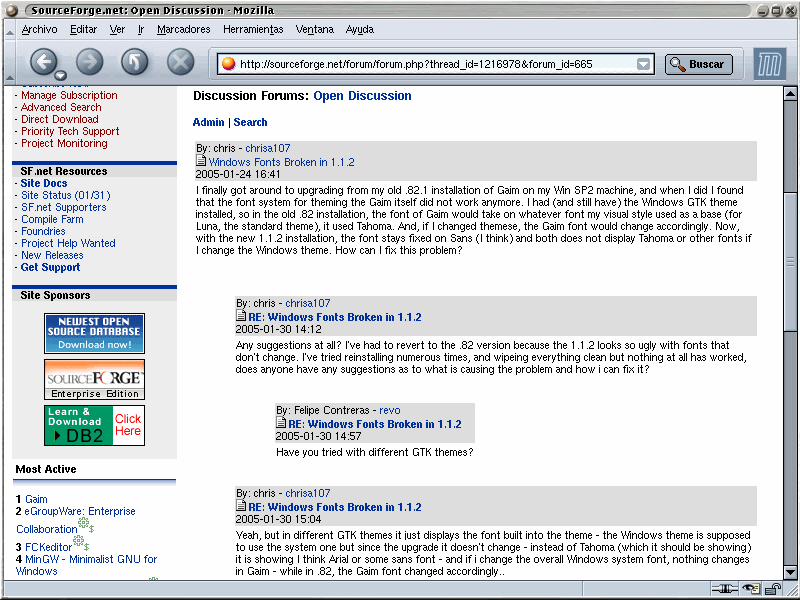
\includegraphics[bb=0 0 800 600, width=12cm, keepaspectratio]{img/foro1}
    \caption{Página con enlaces a hilos}
    \label{figura:foro_hilos}
 \end{figure}


A continuación un bloque ``verbatim'', que se utiliza para mostrar texto tal cual.
Se puede utilizar para ofrecer el contenido de correos electrónicos, código, entre otras cosas.


{\footnotesize
\begin{verbatim}
    From gaurav at gold-solutions.co.uk  Fri Jan 14 14:51:11 2005
    From: gaurav at gold-solutions.co.uk (gaurav_gold)
    Date: Fri Jan 14 19:25:51 2005
    Subject: [Mailman-Users] mailman issues
    Message-ID: <003c01c4fa40$1d99b4c0$94592252@gaurav7klgnyif>

    Dear Sir/Madam,
    How can people reply to the mailing list?  How do i turn off
    this feature? How can i also enable a feature where if someone
    replies the newsletter the email gets deleted?
    Thanks

    From msapiro at value.net  Fri Jan 14 19:48:51 2005
    From: msapiro at value.net (Mark Sapiro)
    Date: Fri Jan 14 19:49:04 2005
    Subject: [Mailman-Users] mailman issues
    In-Reply-To: <003c01c4fa40$1d99b4c0$94592252@gaurav7klgnyif>
    Message-ID: <PC173020050114104851057801b04d55@msapiro>

    gaurav_gold wrote:
    >How can people reply to the mailing list?  How do i turn off
    this feature? How can i also enable a feature where if someone
    replies the newsletter the email gets deleted?

    See the FAQ
    >Mailman FAQ: http://www.python.org/cgi-bin/faqw-mm.py
    article 3.11
\end{verbatim}
}



\section{Estructura de la memoria}
\label{sec:estructura}


\begin{figure}
  \centering
  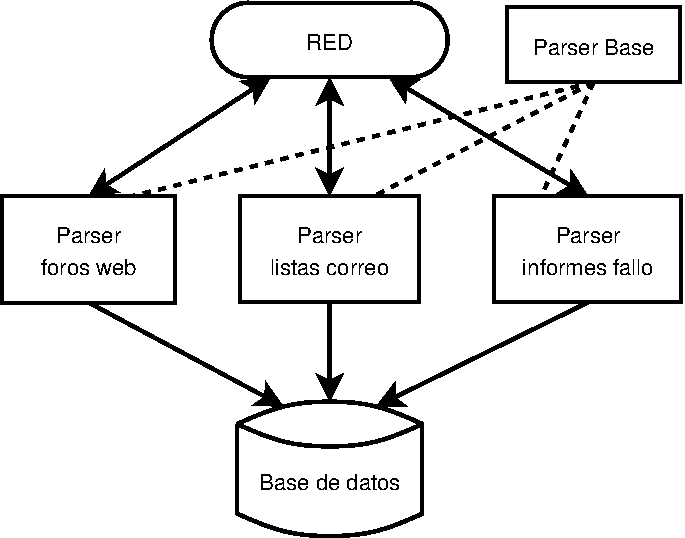
\includegraphics[width=9cm, keepaspectratio]{img/arquitectura.png}
  \caption{Estructura del parser básico}
  \label{fig:arquitectura}
\end{figure}




En esta sección se debería introducir la estructura de la memoria. 

Así:


\begin{itemize}
  \item En el primer capítulo se hace una intro al proyecto.
  
  \item En el capítulo~\ref{chap:objetivos} (ojo, otra referencia automática) se muestran los objetivos del proyecto.
  
  \item A continuación se presenta el estado del arte en el capítulo~\ref{chap:estado}.
  
  \item \ldots
\end{itemize}





%%%%%%%%%%%%%%%%%%%%%%%%%%%%%%%%%%%%%%%%%%%%%%%%%%%%%%%%%%%%%%%%%%%%%%%%%%%%%%%%
%%%%%%%%%%%%%%%%%%%%%%%%%%%%%%%%%%%%%%%%%%%%%%%%%%%%%%%%%%%%%%%%%%%%%%%%%%%%%%%%
% OBJETIVOS %
%%%%%%%%%%%%%%%%%%%%%%%%%%%%%%%%%%%%%%%%%%%%%%%%%%%%%%%%%%%%%%%%%%%%%%%%%%%%%%%%

\cleardoublepage % empezamos en página impar
\chapter{Objetivos} % título del capítulo (se muestra)
\label{chap:objetivos} % identificador del capítulo (no se muestra, es para poder referenciarlo)

\section{Objetivo general} % título de sección (se muestra)
\label{sec:objetivo-general} % identificador de sección (no se muestra, es para poder referenciarla)

Aquí vendría el objetivo general en una frase:
Mi trabajo fin de grado consiste en crear de una herramienta de análisis de los comentarios jocosos en repositorios de software libre alojados en la plataforma GitHub.

Recuerda que los objetivos siempre vienen en infinitivo.


\section{Objetivos específicos}
\label{sec:objetivos-especificos}

Los objetivos específicos se pueden entender como las tareas en las que se ha desglosado el objetivo general.
Y, sí, también vienen en infinitivo.


\section{Planificación temporal}
\label{sec:planificacion-temporal}

A mí me gusta que aquí pongáis una descripción de lo que os ha llevado realizar el trabajo.
Hay gente que añade un diagrama de GANTT.
Lo importante es que quede claro cuánto tiempo llevas (tiempo natural, p.ej., 6 meses) y a qué nivel de esfuerzo (p.ej., principalmente los fines de semana).


%%%%%%%%%%%%%%%%%%%%%%%%%%%%%%%%%%%%%%%%%%%%%%%%%%%%%%%%%%%%%%%%%%%%%%%%%%%%%%%%
%%%%%%%%%%%%%%%%%%%%%%%%%%%%%%%%%%%%%%%%%%%%%%%%%%%%%%%%%%%%%%%%%%%%%%%%%%%%%%%%
% ESTADO DEL ARTE %
%%%%%%%%%%%%%%%%%%%%%%%%%%%%%%%%%%%%%%%%%%%%%%%%%%%%%%%%%%%%%%%%%%%%%%%%%%%%%%%%

\cleardoublepage
\chapter{Estado del arte}
\label{chap:estado}

Descripción de las tecnologías que utilizas en tu trabajo. 
Con dos o tres párrafos por cada tecnología, vale. 
Se supone que aquí viene todo lo que no has hecho tú.

Puedes citar libros, como el de Bonabeau et al., sobre procesos estigmérgicos~\cite{bonabeau:_swarm}. 
Me encantan los procesos estigmérgicos.
Deberías leer más sobre ellos.
Pero quizás no ahora, que tenemos que terminar la memoria para sacarnos por fin el título.
Nota que el \~ \ añade un espacio en blanco, pero no deja que exista un salto de línea. 
Imprescindible ponerlo para las citas.

Citar es importantísimo en textos científico-técnicos. 
Porque no partimos de cero.
Es más, partir de cero es de tontos; lo suyo es aprovecharse de lo ya existente para construir encima y hacer cosas más sofisticadas.
¿Dónde puedo encontrar textos científicos que referenciar?
Un buen sitio es Google Scholar\footnote{\url{http://scholar.google.com}}.
Por ejemplo, si buscas por ``stigmergy libre software'' para encontrar trabajo sobre software libre y el concepto de \emph{estigmergia} (¿te he comentado que me gusta el concepto de estigmergia ya?), encontrarás un artículo que escribí hace tiempo cuyo título es ``Self-organized development in libre software: a model based on the stigmergy concept''.
Si pulsas sobre las comillas dobles (entre la estrella y el ``citado por ...'', justo debajo del extracto del resumen del artículo, te saldrá una ventana emergente con cómo citar.
Abajo a la derecha, aparece un enlace BibTeX.
Púlsalo y encontrarás la referencia en formato BibTeX, tal que así:

{\footnotesize
\begin{verbatim}
@inproceedings{robles2005self,
  title={Self-organized development in libre software:
         a model based on the stigmergy concept},
  author={Robles, Gregorio and Merelo, Juan Juli\'an 
          and Gonz\'alez-Barahona, Jes\'us M.},
  booktitle={ProSim'05},
  year={2005}
}
\end{verbatim}
}

Copia el texto en BibTeX y pégalo en el fichero \texttt{memoria.bib}, que es donde están las referencias bibliográficas.
Para incluir la referencia en el texto de la memoria, deberás citarlo, como hemos hecho antes con~\cite{bonabeau:_swarm}, lo que pasa es que en vez de el identificador de la cita anterior (bonabeau:\_swarm), tendrás que poner el nuevo (robles2005self).
Compila el fichero \texttt{memoria.tex} (\texttt{pdflatex memoria.tex}), añade la bibliografía (\texttt{bibtex memoria.aux}) y vuelve a compilar \texttt{memoria.tex} (\texttt{pdflatex memoria.tex})\ldots y \emph{voilà} ¡tenemos una nueva cita~\cite{robles2005self}!

También existe la posibilidad de poner notas al pie de página, por ejemplo, una para indicarte que visite la página del GSyC\footnote{\url{http://gsyc.es}}.



\section{Sección 1} 
\label{sec:seccion1}

Hemos hablado de cómo incluir figuras.
Pero no hemos dicho nada de tablas.
A mí me gustan las tablas.
Mucho.
Aquí un ejemplo de tabla, la Tabla~\ref{tab:ejemplo} (siento ser pesado, pero nota cómo he puesto la referencia).

\begin{table}
 \begin{center}
  \begin{tabular}{ | l | c | r |} % tenemos tres colummnas, la primera alineada a la izquierda (l), la segunda al centro (c) y la tercera a la derecha (r). El | indica que entre las columnas habrá una línea separadora.
    \hline
    Uno & 2 & 3 \\ \hline % el hline nos da una línea vertical
    Cuatro & 5 & 6 \\ \hline
    Siete & 8 & 9 \\
    \hline
  \end{tabular}
  \caption{Ejemplo de tabla. Aquí viene una pequeña descripción (el \emph{caption}, el pie de tabla/figura) del contenido de la tabla. Si la tabla no es autoexplicativa, siempre viene bien aclararla aquí.}
  \label{tab:ejemplo}
 \end{center}
\end{table}

Hay un sitio en Internet donde puedes diseñar las tablas fácilmente y luego hacer un corta y pega del resultado en tu editor.
Puedes probarlo en \url{https://www.tablesgenerator.com/}.



%%%%%%%%%%%%%%%%%%%%%%%%%%%%%%%%%%%%%%%%%%%%%%%%%%%%%%%%%%%%%%%%%%%%%%%%%%%%%%%%
%%%%%%%%%%%%%%%%%%%%%%%%%%%%%%%%%%%%%%%%%%%%%%%%%%%%%%%%%%%%%%%%%%%%%%%%%%%%%%%%
% DISEÑO E IMPLEMENTACIÓN %
%%%%%%%%%%%%%%%%%%%%%%%%%%%%%%%%%%%%%%%%%%%%%%%%%%%%%%%%%%%%%%%%%%%%%%%%%%%%%%%%

\cleardoublepage
\chapter{Diseño e implementación}
\label{sec:diseno}

Aquí viene todo lo que has hecho tú (tecnológicamente). 
Puedes entrar hasta el detalle. 
Es la parte más importante de la memoria, porque describe lo que has hecho tú.
Eso sí, normalmente aconsejo no poner código, sino diagramas.



\section{Arquitectura general} 
\label{sec:arquitectura}

Si tu proyecto es un software, siempre es bueno poner la arquitectura (que es cómo se estructura tu programa a ``vista de pájaro'').

\begin{figure}
  \centering
  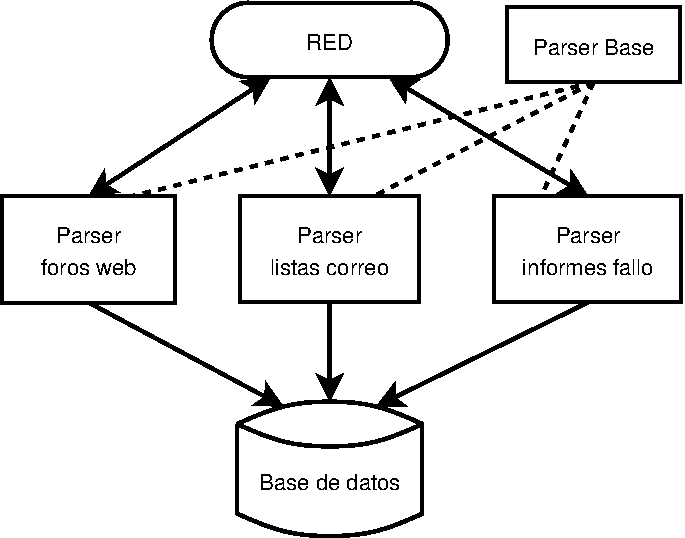
\includegraphics[width=9cm, keepaspectratio]{img/arquitectura.png}
  \caption{Estructura del parser básico}
  \label{fig:arquitectura}
\end{figure}


Por ejemplo, puedes verlo en la figura~\ref{fig:arquitectura}.
\LaTeX \ pone las figuras donde mejor cuadran. 
Y eso quiere decir que quizás no lo haga donde lo hemos puesto\ldots 
Eso no es malo.
A veces queda un poco raro, pero es la filosofía de \LaTeX: tú al contenido, que yo me encargo de la maquetación.


 
Recuerda que toda figura que añadas a tu memoria debe ser explicada.
Sí, aunque te parezca evidente lo que se ve en la figura~\ref{fig:arquitectura}, la figura en sí solamente es un apoyo a tu texto.
Así que explica lo que se ve en la figura, haciendo referencia a la misma tal y como ves aquí.
Por ejemplo: En la figura~\ref{fig:arquitectura} se puede ver que la estructura del \emph{parser} básico, que consta de seis componentes diferentes: los datos se obtienen de la red, y según el tipo de dato, se pasará a un \emph{parser} específico y bla, bla, bla\ldots

Si utilizas una base de datos, no te olvides de incluir también un diagrama de entidad-relación.


%%%%%%%%%%%%%%%%%%%%%%%%%%%%%%%%%%%%%%%%%%%%%%%%%%%%%%%%%%%%%%%%%%%%%%%%%%%%%%%%
%%%%%%%%%%%%%%%%%%%%%%%%%%%%%%%%%%%%%%%%%%%%%%%%%%%%%%%%%%%%%%%%%%%%%%%%%%%%%%%%
% EXPERIMENTOS Y VALIDACIÓN %
%%%%%%%%%%%%%%%%%%%%%%%%%%%%%%%%%%%%%%%%%%%%%%%%%%%%%%%%%%%%%%%%%%%%%%%%%%%%%%%%

\cleardoublepage
\chapter{Experimentos y validación}
\label{chap:experimentos}

Este capítulo se introdujo como requisito en 2019. 
Describe los experimentos y casos de test que tuviste que implementar para validar tus resultados. 
Incluye también los resultados de validación que permiten afirmar que tus resultados son correctos. 


%%%%%%%%%%%%%%%%%%%%%%%%%%%%%%%%%%%%%%%%%%%%%%%%%%%%%%%%%%%%%%%%%%%%%%%%%%%%%%%%
%%%%%%%%%%%%%%%%%%%%%%%%%%%%%%%%%%%%%%%%%%%%%%%%%%%%%%%%%%%%%%%%%%%%%%%%%%%%%%%%
% RESULTADOS %
%%%%%%%%%%%%%%%%%%%%%%%%%%%%%%%%%%%%%%%%%%%%%%%%%%%%%%%%%%%%%%%%%%%%%%%%%%%%%%%%

\cleardoublepage
\chapter{Resultados}
\label{chap:resultados}

En este capítulo se incluyen los resultados de tu trabajo fin de grado.

Si es una herramienta de análisis lo que has realizado, aquí puedes poner ejemplos de haberla utilizado para que se vea su utilidad.


%%%%%%%%%%%%%%%%%%%%%%%%%%%%%%%%%%%%%%%%%%%%%%%%%%%%%%%%%%%%%%%%%%%%%%%%%%%%%%%%
%%%%%%%%%%%%%%%%%%%%%%%%%%%%%%%%%%%%%%%%%%%%%%%%%%%%%%%%%%%%%%%%%%%%%%%%%%%%%%%%
% CONCLUSIONES %
%%%%%%%%%%%%%%%%%%%%%%%%%%%%%%%%%%%%%%%%%%%%%%%%%%%%%%%%%%%%%%%%%%%%%%%%%%%%%%%%

\cleardoublepage
\chapter{Conclusiones}
\label{chap:conclusiones}


\section{Consecución de objetivos}
\label{sec:consecucion-objetivos}

Esta sección es la sección espejo de las dos primeras del capítulo de objetivos, donde se planteaba el objetivo general y se elaboraban los específicos.

Es aquí donde hay que debatir qué se ha conseguido y qué no. 
Cuando algo no se ha conseguido, se ha de justificar, en términos de qué problemas se han encontrado y qué medidas se han tomado para mitigar esos problemas.

Y si has llegado hasta aquí, siempre es bueno pasarle el corrector ortográfico, que las erratas quedan fatal en la memoria final.
Para eso, en Linux tenemos aspell, que se ejecuta de la siguiente manera desde la línea de \emph{shell}:

\begin{verbatim}
  aspell --lang=es_ES -c memoria.tex
\end{verbatim}

\section{Aplicación de lo aprendido}
\label{sec:aplicacion}

Aquí viene lo que has aprendido durante el Grado/Máster y que has aplicado en el TFG/TFM.
Una buena idea es poner las asignaturas más relacionadas y comentar en un párrafo los conocimientos y habilidades puestos en práctica.

\begin{enumerate}
  \item a
  \item b
\end{enumerate}


\section{Lecciones aprendidas}
\label{sec:lecciones_aprendidas}

Aquí viene lo que has aprendido en el Trabajo Fin de Grado/Máster.

\begin{enumerate}
  \item Aquí viene uno.
  \item Aquí viene otro.
\end{enumerate}


\section{Trabajos futuros}
\label{sec:trabajos_futuros}

Ningún proyecto ni software se termina, así que aquí vienen ideas y funcionalidades que estaría bien tener implementadas en el futuro.

Es un apartado que sirve para dar ideas de cara a futuros TFGs/TFMs.


%%%%%%%%%%%%%%%%%%%%%%%%%%%%%%%%%%%%%%%%%%%%%%%%%%%%%%%%%%%%%%%%%%%%%%%%%%%%%%%%
%%%%%%%%%%%%%%%%%%%%%%%%%%%%%%%%%%%%%%%%%%%%%%%%%%%%%%%%%%%%%%%%%%%%%%%%%%%%%%%%
% APÉNDICE(S) %
%%%%%%%%%%%%%%%%%%%%%%%%%%%%%%%%%%%%%%%%%%%%%%%%%%%%%%%%%%%%%%%%%%%%%%%%%%%%%%%%

\cleardoublepage
\appendix
\chapter{Manual de usuario}
\label{app:manual}

Esto es un apéndice.
Si has creado una aplicación, siempre viene bien tener un manual de usuario.
Pues ponlo aquí.

%%%%%%%%%%%%%%%%%%%%%%%%%%%%%%%%%%%%%%%%%%%%%%%%%%%%%%%%%%%%%%%%%%%%%%%%%%%%%%%%
%%%%%%%%%%%%%%%%%%%%%%%%%%%%%%%%%%%%%%%%%%%%%%%%%%%%%%%%%%%%%%%%%%%%%%%%%%%%%%%%
% BIBLIOGRAFIA %
%%%%%%%%%%%%%%%%%%%%%%%%%%%%%%%%%%%%%%%%%%%%%%%%%%%%%%%%%%%%%%%%%%%%%%%%%%%%%%%%

\cleardoublepage

% Las siguientes dos instrucciones es todo lo que necesitas
% para incluir las citas en la memoria
\bibliographystyle{abbrv}
\bibliography{memoria}  % memoria.bib es el nombre del fichero que contiene
% las referencias bibliográficas. Abre ese fichero y mira el formato que tiene,
% que se conoce como BibTeX. Hay muchos sitios que exportan referencias en
% formato BibTeX. Prueba a buscar en http://scholar.google.com por referencias
% y verás que lo puedes hacer de manera sencilla.
% Más información: 
% http://texblog.org/2014/04/22/using-google-scholar-to-download-bibtex-citations/

\end{document}
